\chapter{Propuesta}\label{chapter:proposal}
En el presente capítulo se explica la solución al problema fundamental de este trabajo. Se propone la creación de una \texttt{fabric-chaincode-api} que permita la implementación de contratos inteligentes en el lenguaje $ C\sharp $.

El módulo principal de este proyecto lo constituye el \textit{chaincode shim }pues, expone la interfaz \texttt{IChaincode} al contrato inteligente. Por ello, se dedica la primera sección \ref{chaincodeshim} a analizar sus principales componentes.

La sección \ref{protocolinteraction} describe el protocolo de interacción entre el \textit{chaincode} y el nodo \textit{peer} desde las fases iniciales hasta la ejecución de transacciones.

En la sección \ref{concurrencymodel} se trata el modelo de concurrencia implementado que posibilita procesar varias transacciones a la vez.

Dentro del contexto de una transacción, en ocasiones se hace necesario interactuar con el \textit{ledger}, ya sea para consultas o modificaciones. En este proceso el \textit{peer} actúa como mediador, recibiendo las peticiones del \textit{chaincode} y devolviendo las respuestas. La sección \ref{ledgerinteraction} muestra la propuesta de solución que permite adaptar el proceso \textit{chaincode} a la recepción de dichas respuestas provenientes del \textit{peer}.

%\section{gRPC y \textit{protocol buffers}}
%Como se mencionaba anteriormente, en el \textit{chaincode} se define la lógica de negocio de la aplicación \textit{blockchain} utilizando un lenguaje de programación de propósito general. Los \textit{chaincode} se ejecutan en un entorno desacoplado al resto del nodo \textit{peer}. De esta forma, el \textit{peer} es independiente del lenguaje real en el que se implementa el chaincode. Para cumplir el propósito de este trabajo es necesario implementar un \textit{chaincode} en $ C\sharp$, lenguaje distinto al del nodo peer (Go). En esta sección se explica gRPC  [\cite{grpc-doc}]\footnote{Llamada a Procedimiento Remoto gRPC}, herramienta que permite la comunicación entre ambos elementos. 
%
%En gRPC, una aplicación cliente puede llamar directamente a un método en una aplicación servidor en una máquina diferente como si fuera un objeto local, lo que facilita la creación de aplicaciones y servicios distribuidos que necesitan operar en tiempo real. 

%Como en muchos sistemas RPC, gRPC se basa en la idea de definir un servicio, especificando los métodos que se pueden llamar de forma remota con sus parámetros y tipos de devolución. En el lado del servidor, se implementa una interfaz para manejar las llamadas de los clientes. En el lado del cliente se tiene el \textit{stub}),el cual proporciona los mismos métodos que el servidor.

%La diferencia con otros frameworks RPC existentes radica en la capacidad de gRPC de utilizar \textit{protocol buffers} [\cite{protobuf-doc}] como lenguaje de definición de interfaz para la serialización y como formato de intercambio de mensajes, en lugar de JSON/XML.
%
%Los \textit{protocol buffers} proporcionan un mecanismo extensible, independiente del idioma y de la plataforma, para serializar datos estructurados de manera compatible con versiones anteriores y posteriores. Se pueden ampliar con nueva información sin invalidar los datos existentes ni requerir que se actualice el código.
%
%\begin{figure}[tbph]
%\centering
%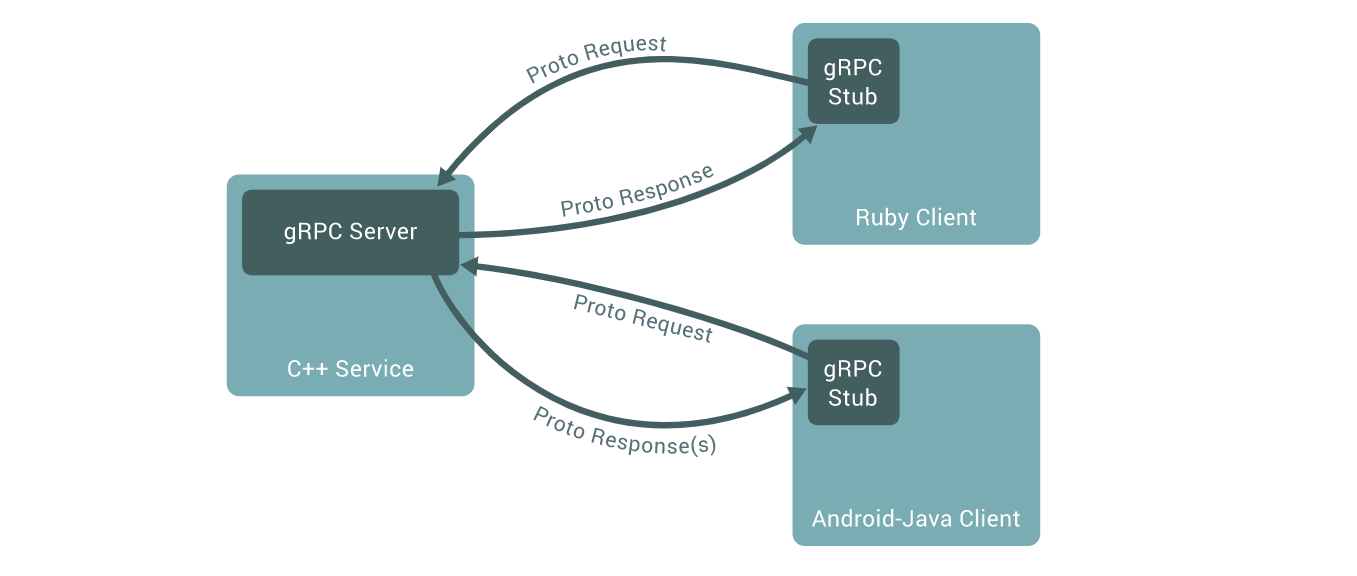
\includegraphics[width=\textwidth]{Images/grpc}
%\caption{ Interacción entre cliente y servidor en gRPC.}
%\label{fig:grpc}
%\end{figure}
%
%Los clientes y servidores de gRPC pueden ejecutarse y comunicarse entre sí en una variedad de entornos y pueden escribirse en cualquiera de los idiomas compatibles con gRPC. La figura \ref{fig:grpc} muestra un ejemplo de servidor gRPC en $ C++ $ con clientes Ruby y Java. En la solución propuesta en este artículo se aprovecha dicha característica para brindar una interfaz de comunicación entre el nodo \textit{peer} y el \textit{chaincode}, escritos en Go y $ C\sharp$ respectivamente.

%\section{fabric-protos-csharp}
%Como se vio en el capítulo anterior, la interacción entre el \textit{chaincode} y el nodo \textit{peer} se establece mediante el intercambio de mensajes \textit{protobuf}.
%El servicio gRPC y las definiciones de \textit{protocol buffers} que se utilizan en Hyperledger Fabric se encuentran en el repositorio \texttt{fabric-protos}, de dominio público. Se empleó la herramienta \texttt{\textbf{protoc}} para compilar estas definiciones al lenguaje C$\sharp$, conformando así el módulo \texttt{fabric-protos-csharp}. Dicha biblioteca provee las clases necesarias para interactuar con Fabric, entre ellas: \texttt{ChaincodeMessage}, \texttt{ChaincodeId}, \texttt{ChaincodeInput}, \texttt{Response}

%Dicha biblioteca provee las clases necesarias para interactuar con Fabric, entre las más utilizadas se encuentran:
%
%\begin{enumerate}
%\item \texttt{ChaincodeMessage:} tipo de los mensajes que se intercambian entre el chaincode y el peer.
%\item \texttt{ChaincodeId:} 
%\item \texttt{ChaincodeInput}
%\item \texttt{GetState}
%\item \texttt{PutState}
%\item \texttt{DelState}
%\item \texttt{Response}
%\end{enumerate}

\section{Chaincode shim} \label{chaincodeshim}

Con el fin de asistir la tarea del desarrollador y centrar sus esfuerzos en implementar la lógica del contrato inteligente, Hyperledger proporciona los \textit{chaincode shims}. Se trata de la implementación del \textit{runtime environment} necesario para integrar el contrato inteligente con Hyperledger Fabric y ejecutarlos como procesos remotos.

%El \textit{shim} es el componente responsable de ejecutar el contrato inteligente, hacerlo accesible para el nodo \textit{peer} y administrar toda la interacción de bajo nivel con él a través de gRPC. Además, proporciona una interfaz simplificada para el contrato inteligente para acceder a los servicios de invocación del \textit{ledger} y el \textit{chaincode} a través del \textit{chaincode stub} [\cite{hlf-internals}].

\begin{figure}[tbph]
\centering
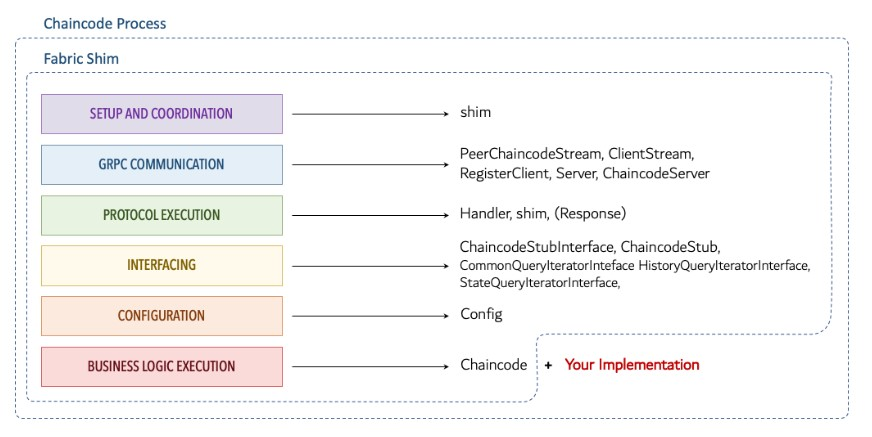
\includegraphics[width=\textwidth]{Images/chaincode_shim}
\caption{Componentes del chaincode shim}
\label{fig:chaincodeshim}
\end{figure}

La figura \ref{fig:chaincodeshim} proporciona un desglose de los componentes que conforman el proceso \textit{chaincode} junto con el rol y las responsabilidades que tiene cada uno en la propuesta de solución que se discute en este documento. Vale la pena señalar que, si bien el \textit{shim} es un componente específico del proceso chaincode, a menos que se especifique lo contrario, el \textit{shim} también se usa para referirse al conjunto de componentes que conforman el proceso chaincode, excepto por la implementación del contrato inteligente.




%\subsection{Patrones de ejecución de Chaincode}
%
% no es necesario construir y lanzar el chaincode para cada \textit{peer}.
%\end{enumerate}

\section{Protocolo de interacción}\label{protocolinteraction}
El \textit{shim} de Fabric admite dos modalidades de ejecución, que controlan el comportamiento de la conexión entre el \textit{chaincode} y el nodo \textit{peer}:

\begin{enumerate}
\item \textbf{Chaincode como cliente:} esta es la modalidad por defecto y la única utilizada en Hyperledger Fabric v1.4 [\cite{hlf-internals}]. Presenta el proceso \textit{chaincode} como un cliente que inicia la conexión con el \textit{peer}.

\item \textbf{Chaincode como servidor:} A partir de la versión 2.0, Hyperledger Fabric admite la implementación de \textit{chaincode} fuera de la blockchain [\cite{hlf-internals}]. De esta forma, el \textit{chaincode} se ejecuta como un servidor independiente del \textit{peer}.
\end{enumerate}

En este escenario, la inicialización admite el patrón \textbf{chaincode como  servidor}.\\[10cm]

%El \textit{shim} también tiene la capacidad de inicializarse para admitir el patrón \textbf{chaincode como cliente}, donde los roles se invierten.



\begin{figure}[tbph]
\centering
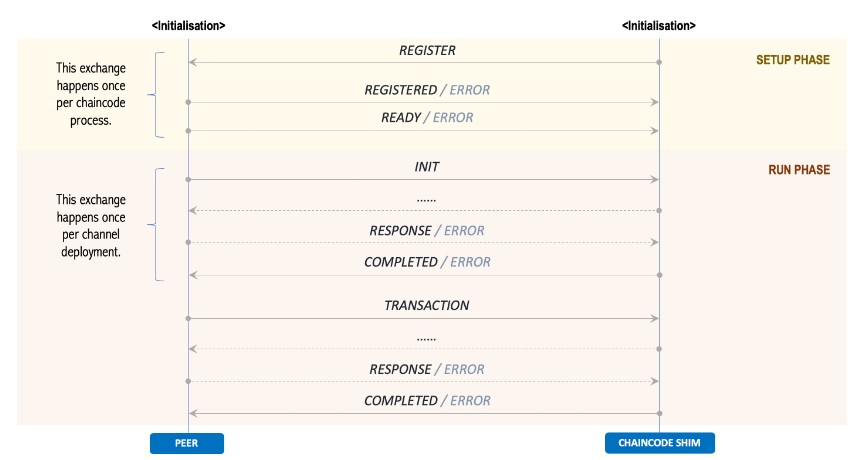
\includegraphics[width=\textwidth]{Images/interaction_protocol}
\caption{Interacción entre el nodo \textit{peer} y el \textit{chaincode shim}}
\label{fig:interactionprotocol}
\end{figure}

La figura \ref{fig:interactionprotocol} proporciona una descripción general del protocolo de interacción de extremo a extremo, el cual se lleva a cabo a través del intercambio de mensajes \textit{\textbf{protobuf}}.

El ciclo de vida de la interacción se desarrolla en tres fases: \textbf{inicialización}, \textbf{configuración} y \textbf{ejecución de la transacción} (o fase de ejecución). En las siguientes secciones se proporcionarán detalles para cada una.

\subsection{Fase 1: Inicialización}
%Durante la fase de inicialización, el \textit{peer} realiza una serie de operaciones:
%
%\begin{enumerate}
%
%\item Inicializa un objeto \texttt{ChaincodeSupport} que expone los servicios del \textit{chaincode} al nodo \textit{peer}.
%
%\item Inicia un servidor gRPC de tipo \texttt{ChaincodeSupportServer} y registra el servicio \texttt{ChaincodeSupport} para habilitar la interacción con los procesos del \textit{chaincode}.
%
%\item Inicia un servidor gRPC de tipo \texttt{EndorserServer}  para recibir propuestas de transacción para ser aprobadas.
%\end{enumerate}

En la fase de iniciaización, el \textit{shim} llama la función  \texttt{ChaincodeServer.Start()}, encargada de realizar las siguientes operaciones:

\begin{enumerate}
\item Inicialización del servidor gRPC, utilizado para conectarse con el \textit{peer} y configurar un flujo bidireccional para intercambiar instancias de \texttt{ChaincodeMessage}.

%\item \textbf{Inicialización del \textit{handler}:} este componente se encarga de procesar todos los mensajes enviados por el \textit{peer} y ejecutar las operaciones asociadas.

\item Registra el servicio \texttt{Connect} para habilitar la interacción con los procesos del \textit{peer}.

\item Levanta el servidor gRPC inicializado anteriormente  para recibir propuestas de transacción.
%\item \textbf{Inicialización del ciclo de procesamiento de mensajes:} este se utiliza para recibir los mensajes del \textit{peer} y enviarlos al \textit{handler} para su posterior procesamiento.
\end{enumerate}

\subsection{Fase 2: Configuración}
Antes de iniciar el ciclo para recibir de mensajes, el \textit{shim} crea una instancia de \textit{Handler} para manejar el intercambio de mensajes con el proceso del \textit{chaincode}. Luego, envía un mensaje \texttt{REGISTER} a través del flujo bidireccional abierto con el \textit{peer}. Este mensaje contiene los detalles del \textit{chaincode} para registrarse codificado como \texttt{ChaincodeID}. Al recibir el mensaje, el \textit{peer} valida la información asociada al \textit{chaincode} y responde con un mensaje \texttt{REGISTERED} e inmediatamente después con un mensaje \texttt{READY}, lo que indica la finalización del proceso de configuración.

\subsection{Fase 3: Ejecución de la transacción}
Una vez que se completa la fase de configuración, el \textit{chaincode} y el \textit{peer} están listos para ejecutar transacciones.

A partir de este punto, la interacción es impulsada por el \textit{peer}, como resultado de las operaciones que envían los clientes de la aplicación al mismo. Por lo general, implican el despliegue del \textit{chaincode} en un canal específico y la posterior invocación de transacciones en el contrato inteligente implementado.

\begin{figure}[tbph]
\centering
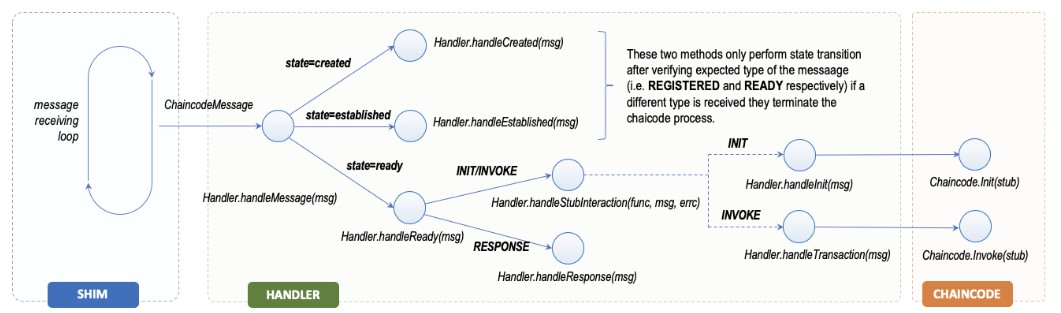
\includegraphics[width=\textwidth]{Images/interaction_flow}
\caption{Flujo de interacción entre \textit{peer}, \textit{handler} y \textit{chaincode}}
\label{fig:interactionflow}
\end{figure}

La figura \ref{fig:interactionflow} muestra el flujo de interacción entre el \textit{shim}, el \textit{handler} y la implementación de \texttt{Chaincode} durante el procesamiento de una propuesta de transacción. El bucle de mensajes implementado en el método \texttt{Connect()} envía el mensaje al \textit{handler} que, en función de su estado, lo procesa. 
%
%La ruta más relevante para estos flujos es lo que sucede cuando el \textit{handler} está en estado \texttt{READY} y procesa invocaciones de transacciones a través del método \texttt{handleTransaction(ChaincodeMessage msg)} o respuestas a solicitudes al \textit{peer} por parte del chaincode a través del método\texttt{ handleResponse(ChaincodeMessage msg)}.







%Esta interacción se implementa en los siguientes pasos:
%
%\begin{enumerate}
%\item Como resultado del despliegue del \textit{chaincode}, el \textit{peer} envía un mensaje \texttt{INIT}. 
%
%%El \textit{handler} inicializa un contexto de transacción para la simulación de la propuesta de transacción asociada a la inicialización y envía el mensaje a través de un flujo bidireccional.
%
%\item Tras la recepción del mensaje \texttt{INIT}, el \textit{handler} crea una nueva instancia de \texttt{ChaincodeStub}, que representa la interfaz para los servicios expuestos al contrato inteligente. Luego se invoca \texttt{Chaincode.Init()} pasando el \textit{stub} como argumento.
%
%\item El \textit{chaincode} ejecuta la inicialización del contrato inteligente y el método \texttt{Init()} se completa con éxito o con un error. El primero hace que se envíe un mensaje \texttt{COMPLETED} al \textit{peer}, mientras que el segundo provoca un mensaje de \texttt{ERROR}.

%\item Al recibir el mensaje, el \textit{peer} invoca el método \texttt{Handler.Notify()} en la instancia asociada al \textit{chaincode}. Este método cierra el contexto de transacción previamente abierto y hace que el método \texttt{Handler.Execute()} desbloquee y devuelva la respuesta obtenida por el \textit{chaincode}.

%\end{enumerate}

%Las invocaciones posteriores del mismo \textit{chaincode} en el mismo canal dan como resultado que el \textit{peer} envíe un mensaje \texttt{TRANSACTION}, que se maneja de la misma manera que se detalla para el mensaje \texttt{INIT}.

La ejecución de la propuesta de transacción se lleva a cabo a través del método \texttt{Handler.HandleReady()} descrito en el código \ref{code:handleReady}. Este se encarga de enviar los mensajes según su tipo a la función del \textit{handler} adecuada.\\


\begin{lstlisting}[escapeinside={(*}{*)}, caption={Función \texttt{Handler.HandleReady()}}, label={code:handleReady}]
public async void HandleReady(ChaincodeMessage chaincodeMessage)  
{
  switch (chaincodeMessage.Type)
    {
	    case ChaincodeMessage.Types.Type.Response:
	        _messageQueue.HandleMessageResponse(chaincodeMessage);
	        break;
	
	    case ChaincodeMessage.Types.Type.Init:
	        await HandleInit(chaincodeMessage);
	        break;
	
	    case ChaincodeMessage.Types.Type.Transaction:
	        await HandleTransaction(chaincodeMessage);
	        break;
    }
}
\end{lstlisting}

Se manejan tres casos diferentes, dos de ellos dan como resultado la ejecución asíncrona de los métodos del \textit{chaincode}: \texttt{chaincode.Init()} y \texttt{chaincode.Invoke()}. El procesamiento de los mensajes \texttt{RESPONSE} del \textit{peer} se maneja dentro del mismo hilo.\\

La tramitación de los dos tipos de propuestas se deja a las siguientes funciones:\\

\begin{lstlisting}
	public async Task HandleInit(ChaincodeMessage msg) {...}
	public async Task HandleTransaction(ChaincodeMessage msg) {...}
\end{lstlisting}

Estas funciones tienen esencialmente la misma lógica que comprende los siguientes pasos:

\begin{enumerate}
\item Deserialización de la instancia \texttt{ChaincodeInput} a partir de la información en \texttt{ChaincodeMessage}.

\item Creación de una nueva instancia \texttt{ChaincodeStub} y configuración del contexto de transacción que comprende: identificador de canal, identificador de transacción, entrada (es decir, \texttt{ChaincodeInput}) y propuesta firmada (\textit{signed proposal}).

\item Invocación del método \texttt{Chaincode.Init()} o \texttt{Chaincode.Invoke()}.
\end{enumerate}

Si hay un error de invocación el método devolverá un \texttt{ChaincodeMessage} de tipo \texttt{ERROR}, si la ejecución es exitosa devolverá un mensaje de tipo \texttt{COMPLETED} conteniendo la respuesta producida por el \textit{chaincode}.


%\section{Flujo de interacción}

\section{Procesamiento concurrente de transacciones}\label{concurrencymodel}
La figura \ref{fig:concurrencyModel} muestra una vista del modelo de concurrencia implementado en el \textit{shim}. Por simplicidad, las diferentes rutas de ejecución que se ejecutan simultáneamente se denominan hilos, independientemente de su implementación subyacente (es decir, hilos, Tasks, etc). Dentro de este contexto, el término se usa simplemente para referirse a una función ejecutada simultáneamente con otras.

\begin{figure}[tbph]
\centering
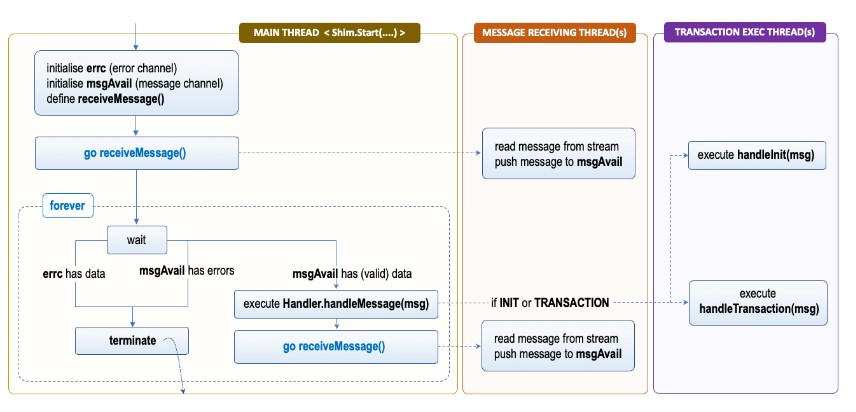
\includegraphics[width=\textwidth]{Images/concurrency_model}
\caption{Modelo de concurrencia}
\label{fig:concurrencyModel}
\end{figure}

Hay tres hilos principales que definen el flujo:

\begin{enumerate}
\item \textbf{Hilo principal:} ejecuta el punto de entrada del proceso chaincode, es responsable de su inicialización e implementa el bucle infinito que envía los mensajes al handler. Este hilo es responsable del ciclo de vida del proceso general y si se detecta algún error inesperado en la recepción de mensajes o el procesamiento de propuestas, finaliza el proceso.

\item \textbf{Hilo de recepción de mensajes:} este hilo ejecuta la función que escucha el flujo bidireccional establecido con el peer y deserializa los datos entrantes en forma de instancias de \texttt{ChaincodeMessage}. 

%Luego, estos se envían a través del canal msgAvail al hilo principal para su posterior procesamiento. Tanto los datos válidos como los errores se pasan a través del canal msgAvail.

\item \textbf{Hilo de ejecución de transacciones:} ejecuta la simulación de la propuesta de transacción, ya sea mediante la invocación de \texttt{handleInit(ChaincodeMessage)} o \texttt{handleTransaction(ChaincodeMessage)}

\end{enumerate}
Este modelo de ejecución permite que el proceso del \textit{chaincode} aumente el rendimiento pues, las propuestas de transacción se ejecutan de forma asíncrona, lo que deja libre al hilo principal para procesar otras solicitudes.

\section{Interacción con el ledger}\label{ledgerinteraction}
Un requisito común de los desarrolladores de contratos inteligentes es poder consultar el \textit{ledger} dentro del contexto de una transacción, ya sea para leer o escribir en el mismo. Como el diseño del contrato inteligente es esencialmente \textit{stateless}, cualquier información adicional que no venga con los argumentos del \textit{chaincode} debe leerse del \textit{ledger}. Esta invocación está mediada por el \textit{peer} y, por lo tanto, es necesario establecer una comunicación con el mismo dentro del contexto de una transacción.

Para resolver este problema se tiene en el \textit{handler} una instancia de la clase \texttt{MessageQueue}, expuesta en el código \ref{code:messagequeue}.

\begin{lstlisting}[escapeinside={(*}{*)}, caption={Clase MessageQueue}, label={code:messagequeue}]
public class MessageQueue : IMessageQueue
{
    private readonly IHandler _handler;

    private readonly ConcurrentDictionary<string, ConcurrentQueue<QueueMessage>> _txQueues =
        new ConcurrentDictionary<string, ConcurrentQueue<QueueMessage>>();

    public MessageQueue(IHandler handler){}

    public Task QueueMessage(QueueMessage queueMessage){}

    public void HandleMessageResponse(ChaincodeMessage response){}

    private Task SendMessage(string messageTxContextId){}

    private QueueMessage GetCurrentMessage(string messageTxContextId){}

    private void RemoveCurrentAndSendNextMessage(string messageTxContextId){}

    private void HandleResponseMessage<T>(
        QueueMessage<T> message,
        string messageTxContextId,
        ChaincodeMessage response
    ){}
}
\end{lstlisting}
La propiedad \texttt{txQueues} provee un diccionario que asocia una llave con una cola de mensajes de tipo \texttt{QueueMessage}. Esta llave es resultado de concatenar el identificador de canal (\texttt{ChannelId}) y el identificador de transacción (\texttt{TxId}), por tanto, es única para cada transacción.

Dado que las invocaciones a transacciones se realizan de forma concurrente, varios hilos van a necesitar acceder al diccionario al mismo tiempo. Por ello, se utiliza la clase \texttt{ConcurrentDictionary<TKey,TValue>} pues, representa una colección a la que pueden acceder varios hilos a la vez de forma segura [\cite{microsoftdoc}].

Cada vez que se necesite mandar un mensaje al \textit{peer} se llama al método \texttt{AskPeerAndListen()} representado en el código \ref{code:askpeer}. Este se encarga de añadir el mensaje a la cola correspondiente y crea un \texttt{Task} que permanecerá bloqueado hasta que el \textit{peer} devuelva la respuesta. 

\begin{lstlisting}[caption={Función \texttt{Handler.AspPeerAndListen<T>(...)}}, label={code:askpeer}]
private Task<T> AskPeerAndListen<T>(ChaincodeMessage message, MessageMethod method)
{

	var taskCompletionSource = new TaskCompletionSource<T>();
	
	var queueMessage = new QueueMessage<T>(message, method, taskCompletionSource);
	_messageQueue.QueueMessage(queueMessage);
	
	return taskCompletionSource.Task;
}
\end{lstlisting}


Como se muestra en el código \ref{code:handleReady}, al recibir un mensaje tipo \texttt{RESPONSE}, el \textit{handler} llama al método\texttt{ HandleMessageResponse(response)}. Este procede a deserializar la respuesta y devolverla al \texttt{Task} correspondiente, lo que provoca el cierre del mismo. Luego, se elimina el mensaje de la cola y se manda el siguiente a través del método 
\texttt{RemoveCurrentAndSendNextMessage()} presentado en el código \ref{code:sendnextmessage}.\\

\begin{lstlisting}[caption={Función \texttt{RemoveCurrentAndSendNextMessage(...)} }]
 private void RemoveCurrentAndSendNextMessage(string messageTxContextId)
{
    if (!_txQueues.TryGetValue(messageTxContextId, out var messageQueue) || messageQueue.Count <= 0) return;

    messageQueue.TryDequeue(out _);

    if (messageQueue.Count == 0)
    {
        _txQueues.TryRemove(messageTxContextId, out _);
        return;
    }

    SendMessage(messageTxContextId);
}
\end{lstlisting}

Nótese que este procedimiento no impone restricciones al desarrollador del contrato inteligente pues, pueden existir varios hilos dentro de una misma transacción usando funciones que requieran del \textit{peer}. Los mensajes se añadirán a la cola correspondiente y se enviarán uno a la vez, de forma que al recibir la respuesta del \textit{peer} esta sólo puede corresponder al último mensaje enviado.

